\section{Lines, Slope, and Functions} \label{S:0.1.Functions}


\vspace*{-14 pt}
\framebox{\hspace*{3 pt}
\parbox{6.25 in}{\begin{goals}
\item What is a function and what do we mean by its domain and range?
\item What is the slope of a line? What are linear functions and families of linear
    functions?
\end{goals}} \hspace*{3 pt}}

% \begin{web}
% \item
%     \href{https://www.youtube.com/watch?v=AfoNnJ038zA&list=PL9bIjQJDwfGuXQHuS5Jkmum_CFILoCZX-&index=92}{Video:
%     How to read a math textbook}
% \item
%     \href{https://www.khanacademy.org/math/algebra/solving-linear-equations-and-inequalities}{Khan
%     Playlist: Linear Equations}
% \item \href{https://www.khanacademy.org/math/algebra/algebra-functions}{Khan Playlist:
%     Functions}
% \item \href{https://www.khanacademy.org/math/algebra2/functions_and_graphs}{Khan Playlist:
%     Functions and Graphs}
% \end{web}

\nin \hrulefill



\subsection*{Introduction}
We begin our study of calculus by reminding the reader of several pre-requisite topics.
The study of calculus depends on a thorough understanding of these topics and it is
imperative that the reader become as familiar as possible with these topics.  In the
present section we remind the reader about the concepts of functions, slope, and lines,
but first, there are a few things that you should do to get your self ready to use this
text.

\begin{pa} \label{PA:0.1}
    This is the first Preview Activity in this text.  Your job for this activity is to get
    to know the textbook.
    \ba
    \item Where is the full textbook stored?  Find it and save a copy to your computer.
    \item What chapters of this text are you going to cover this semester.  Have a look at
        your syllabus!
%     \item There are a few appendices in the textbook.  What are they and 
%         where are they?
    \item What are the differences between Preview Activities, Activities, Examples,
        Exercises, Voting Questions, and WeBWork?  Which ones should you do before class,
        which ones will you likely do during class, and which ones should you be doing
        after class?
    \item What materials in this text would you use to prepare for an exam and where do
        you find them?
    \item What should you bring to class every day?
    \ea
\end{pa} \afterpa


\subsection*{Functions}
Let's start with the fundamental mathematical idea of a function.  
\begin{definition}[Function]
    A function is a mathematical rule that assigns exactly one output for every
    input.  
\end{definition}

It is easy to give many common examples of functions:
\begin{itemize}
    \item The area of a circle $A$ is a function of the radius of the circle:  $A(r)= \pi r^2$.
    \item The amount $M$ in your savings account is a function of the rate of interest the
        bank pays.
    \item The fuel efficiency in your car is a function of many things, e.g. the speed at
        which you drive, the number of cylinders in your engine, the type of driving
        conditions, etc.
    \item The pressure on a diver is a function of the depth of the diver under water.
\end{itemize}

\begin{definition}[Domain of a Function]
    The domain is the set of all possible inputs for a function.
\end{definition}

\begin{definition}[Range of a Function]
    The range is the set of all possible outputs for a function.
\end{definition}

\bex
Find the domain and range of the functions $f(x) = \sin(x), g(x) = \sqrt{x},$ and $h(x) =
    \frac{1}{x}$.
\eex
For $f(x)=\sin(x)$ we recall that the sine function is defined for every possible value of $x$ but
the output is strictly between $y=-1$ and $y=1$.  Therefore, the domain for $f(x) =
\sin(x)$ is $-\infty < x < \infty$ and the range is $-1 \le y \le 1$.  See the left plot
in Figure \ref{f:0.1ex1}.

For $g(x) = \sqrt{x}$ we recall that the square root of a negative number results in an
imaginary number.  In this text we are interested in real-valued output for functions so
we must omit all of the negative numbers from the domain and hence $0 \le x < \infty$.
For the range we recall that the square root of a number will always be a non-negative
number.  As such, the range is $0 \le y < \infty$.  See the middle plot
in Figure \ref{f:0.1ex1}.

For $h(x) = \frac{1}{x}$ we recall that division by zero is mathematically impossible.
That is the only troublesome point in the domain so $-\infty < x < 0$ or $0 < x < \infty$.
A moment's reflection also reveals that it is impossible to get zero out of the function
$h(x)$ but it is possible to get any other number.  Hence $-\infty < y < 0$ or $0 < y <
\infty$. See the right plot in Figure \ref{f:0.1ex1}. 
\afterex
\begin{figure}
    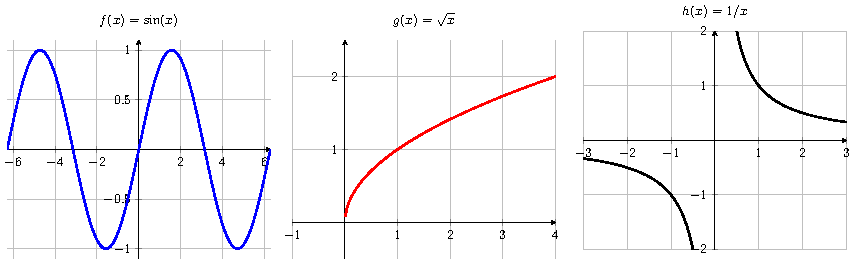
\includegraphics[width=0.95\columnwidth]{figures/0-1-ex1.pdf}
    \caption{Graphs of the function $f(x) = \sin(x)$, $g(x) = \sqrt{x}$, and $h(x) =
    \frac{1}{x}$.}
    \label{f:0.1ex1}
\end{figure}

% It is often convenient to examine functions graphically instead of algebraically.  In our
% previous example we 
% 
% Probably the most common method for representing a function is with a graph.  If the
% domain of function $f$ is set $A$, then the graph of $f$ is the collection of all ordered
% pairs of the form $(x,f(x))$ where $x$ comes from the domain $A$.

It is also important to recall the notation for functions.  When we write $f(x) =
\sqrt{x}$ we are saying several things.  First, the ``$f$'' is the name of the function
that we're defining.  The naming convention gives us a convenient way to refer to
functions without having to explicitly state their algebraic form.  Next, the ``$(x)$'' is
an explicit statement to the reader that the variable ``$x$'' is the independent variable
for the function $f$.  Lastly, the right-hand side of the definition tells us exactly what
to do with the independent variable algebraically.  

When we write $f(25)$ we are referring to the already defined function $f$ and explicitly
saying to replace the independent variable with the number $25$.  In this instance, $f(25)
= \sqrt{25} = 5$.  Similarly, if we write $f(\sin(x))$ we mean to find the independent
variable $x$ in the function $f$ and replace it with the function $\sin(x)$.  In this
case, $f(\sin(x)) = \sqrt{\sin(x)}$.  This is simply a new function.

A function does not always need to be given algebraically.  The three primary
representations of a function are the algebraic form, the graphical form, and the tabular
form.  For example, for the function $f(x) = \sqrt{x}$ we are explicitly giving the
algebraic form and the middle plot of Figure \ref{f:0.1ex1} shows the graphical form.
Table \ref{t:0.1ex1} shows a portion of the table of values.  The distinct disadvantage
for a table of values on many functions is that there are infinitely many possible input
values and a table can naturally only show finitely many of them.

\begin{table}[ht!]
    \centering
    \begin{tabular}{|c||c|c|c|c|c|c|}
        \hline
        $x$ & 0 & 1 & 2 & 3 & 4 & 5 \\ \hline
        $f(x)$ & 0 & 1 & 1.414 & 1.732 & 2 & 2.236 \\ \hline
    \end{tabular}
    \caption{Tabular form of the function $f(x) = \sqrt{x}$.}
    \label{t:0.1ex1}
\end{table}


\begin{activity}\label{A:0.1.1}
The graph of a function $f(x)$ is shown in the plot below. 

\begin{minipage}{0.5\columnwidth}
\begin{center}
%     \begin{tikzpicture}
%         \begin{axis}[axis lines=center, xmin=-1, xmax=5, ymin=-7, ymax=4, grid,
%             xlabel={$x$}, ylabel={$y$}, title={Graph of $f(x)$}]
%             \addplot[smooth, blue, very thick, domain=0:4] {0.5*x*(x+1)*(x-2)*(x-4)};
%             \draw[fill=blue] (axis cs:0,0) circle(0.05cm);
%             \draw[fill=blue] (axis cs:4,0) circle(0.05cm);
%             \draw[fill=blue] (axis cs:1,3) circle(0.05cm) node[anchor=south]{$(1,3)$};
%             \draw[fill=blue] (axis cs:3,-6) circle(0.05cm) node[anchor=north east]{$(3,-6)$};
%         \end{axis}
%     \end{tikzpicture}
    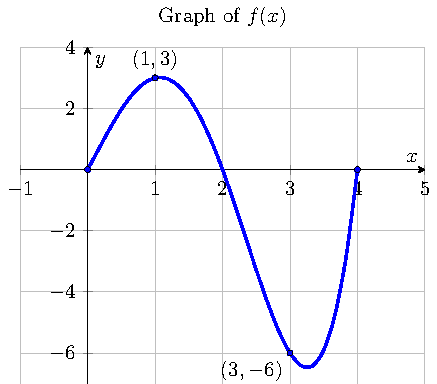
\includegraphics[width=0.9\columnwidth]{figures/0-1-act1.pdf}
\end{center}
\end{minipage}
\begin{minipage}{0.5\columnwidth}
\ba
\item What is the domain of $f(x)$?
\item Approximate the range of $f(x)$.
\item What are  $f(0)$, $f(1)$, $f(3)$, $f(4)$, and $f(5)$?
\ea
\end{minipage}

\end{activity}
\begin{smallhint}
    \ba
        \item The domain is the collection of possible $x$ values.
        \item The range is the collection of possible $y$ values.
        \item Find the $y$ values for each of the given $x$ values.
    \ea
\end{smallhint}
\begin{bighint}
    \ba
        \item The domain should be written as $?? \le x \le ??$.  Look for the smallest
            and largest possible $x$ values.
        \item The range should be written as $?? \le y \le ??$.  Approximate the smallest
            and largest possible $y$ values.
        \item Find the $y$ values for each of the given $x$ values.
    \ea
\end{bighint}
\begin{activitySolution}
   \ba
        \item The domain of $f(x)$ is $0 \le x \le 4$.
        \item The approximate range of $f(x)$ is $-7 \le y \le 3$.  Without the function
            itself we cannot be sure of the actual heights of the function at the maximum
            and the minimum.
        \item $f(0) = 0$, $f(1) = 3$, $f(3) = -6$, $f(4) = 0$, and $f(5)$ does not exist
            since $5$ is not in the domain of $f(x)$.
   \ea
\end{activitySolution}
\aftera




\subsection*{Slope and Linear Functions}
One of the basic graphical ideas of calculus is that if we zoom in close enough to a
curved function it will look approximately linear.  The words ``zoom'' and ``close
enough'' will be made explicit later.  We now review the features of linear functions so
that the idea of ``zoomed in linearity'' can flow naturally later in the course.  

Every linear function is characterized by a constant rate of change; the slope.  The slope
of a linear function is a measure of the ``steepness'' of the line.  We use the symbols
$\Delta x$ and $\Delta y$ which mean respectively the ``change in $x$'' and the ``change in
$y$''.  
\begin{definition}[slope]
    The slope, $m$ of a (non-vertical) linear function $f$ which passes through any
    two points $(x_1,y_1)$, $(x_2,y_2)$ can be found using the formula
    \[ m = \frac{\Delta y}{\Delta x} = \frac{y_2 - y_1}{x_2 - x_1} =
    \frac{f(x_2)-f(x_1)}{x_2-x_1} = \frac{\text{Rise}}{\text{Run}} \]
\end{definition}

As shown in Figure \ref{f:0.1slope}, the slope of a linear function has the following characteristics:
\begin{itemize}
    \item if the line rises from left to right then the slope is positive,
    \item if the line falls from left to right then the slope is negative,
    \item if the line is horizontal then the slope is zero, and
    \item if the line is vertical then the slope is undefined.
\end{itemize}
\begin{figure}
    \begin{center}
%         \begin{tikzpicture}[scale=0.8]
%             \draw[<->, thick] (-4,0) -- (4,0) node[anchor=west]{$x$};
%             \draw[<->, thick] (0,-2) -- (0,4) node[anchor=south]{$y$};
%             \draw[<->, very thick, blue] (-4,3) -- (4,-1) node[anchor=west]{Negative
%             Slope};
%             \draw[<->, very thick, color=red, dashed] (-4,-2) -- (4,3)
%             node[anchor=west]{Positive Slope};
%             \draw[<->, very thick, color=black, dotted] (-4,2) -- (4,2)
%             node[anchor=west]{Zero Slope};
%         \end{tikzpicture}
        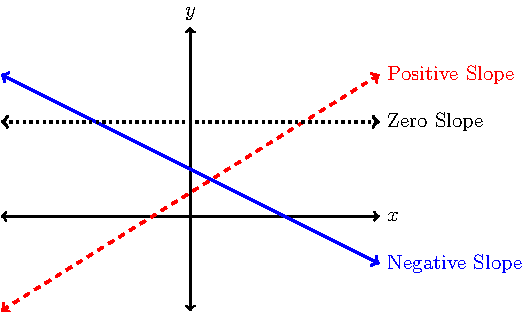
\includegraphics[width=0.6\columnwidth]{figures/0-1-fig3.pdf}
    \end{center}
    \caption{Characteristics of slope.}
    \label{f:0.1slope}
\end{figure}

Depending on the information given there are several convenient forms of the equation of a
line.  Given the definition of the slope
\[ m = \frac{y_2 - y_1}{x_2 - x_1} \]
and letting $(x,y) = (x_2,y_2)$ be any arbitrary point we get the point-slope form of a
linear function by observing that $m = \frac{y - y_1}{x - x_1}$ which implies
that $y - y_1 = m(x-x_1)$.
\begin{definition}[point-slope form of a line]
If the linear function $f$ has slope $m$ and passes through the
point $(x_1,y_1)$, then the point-slope form of the equation of a line is given by: 
\[ y-y_1=m(x- x_1).  \]
\end{definition}

An alternate form of a linear function which is probably very familiar to most readers is
the slope-intercept form of a line.
\begin{definition}[slope intercept form of a line]
If the linear function $f$ has slope $m$ and $y$-intercept $b$, then the
slope-intercept form of the equation of a line is given by: 
\[ y=mx + b.  \]
\end{definition}
In a calculus class the point-slope form is often the most useful.  If you have a linear
function written in the point-slope form you can always rearrange to get it into the
slope-intercept form
\[ y - y_1 = m(x-x_1) \quad \implies \quad y = mx - m x_1 + y_1. \]
Hence we see that the $y$ intercept of a line can be given as $b = -mx_1 + y_1$.
The
symbols and geometry used in each of the above definitions are shown in Figure
\ref{fig:0.1.linear_fn}.

\begin{figure}[ht!]
    \centering
%     \begin{tikzpicture}
%         \draw[color=gray!50] (-4,-2) grid (4,4);
%         \draw[<->, thick] (-4,0) -- (4,0) node[anchor=west]{$x$};
%         \draw[<->, thick] (0,-2) -- (0,4) node[anchor=south]{$y$};
%         \draw[<->, very thick, blue] (-4,3) -- (4,-1);
%         \draw[color=black, fill=black] (-3.5,2.75) circle(0.075cm) node[anchor=south
%         west]{$(x_1,y_1)$};
%         \draw[color=black, fill=black] (-1,1.5) circle(0.075cm) node[anchor=south
%         west]{$(x_2,y_2)$};
%         \draw[color=black, fill=black] (0,1) circle(0.075cm) node[anchor=south
%         west]{$(0,b)$};
%         \draw[thick, dashed] (-3.5,2.75) -- (-3.5,1.5) -- (-1,1.5);
%         \draw (-3.5,2.25) node[anchor=east]{Rise$=\Delta y$};
%         \draw (-2,1.5) node[anchor=north]{Run$=\Delta x$};
%     \end{tikzpicture}
    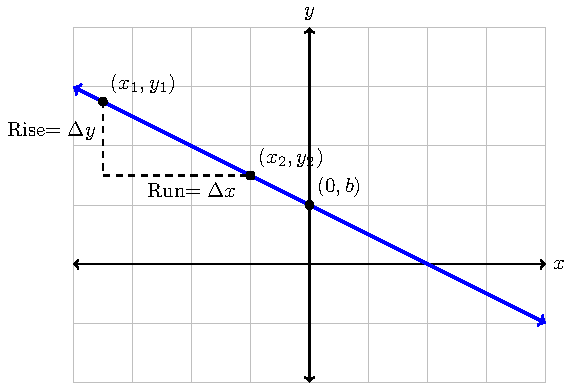
\includegraphics[width=0.6\columnwidth]{figures/0-1-fig4.pdf}
    \caption{Anatomy of a linear function.}
    \label{fig:0.1.linear_fn}
\end{figure}


\begin{activity}\label{A:0.1.2}
Find an equation of the line with the given information.
\ba
\item The line goes through the points $(-2,5)$ and $(10,-1)$.
\item The slope of the line is $3/5$ and it goes through the point $(2,3)$.
\item The $y$-intercept of the line is $(0,-1)$ and the slope is $-2/3$.
\ea

\end{activity}\aftera


\bex
Write the equation of the line going through the points $(5,7)$ and $(-3,2)$.
\eex
First we calculate the slope 
\[ m = \frac{\Delta y}{\Delta x} = \frac{7 - 2}{5-(-3)} = \frac{5}{8}. \]
Since we have two points and neither is the $y$ intercept of the linear function we choose
to use the point-slope form of the line.  Letting $(x_1,y_1) = (5,7)$ we see that
\[ y - 7 = \frac{5}{8} \left( x-5 \right) \]
is one form of the linear function.  
It is often conventient to solve for $y$ giving us
\[ y = \frac{5}{8} \left( x-5 \right) + 7. \]
Notice that we do not necessarily need to simplify all the way to the slope-intercept form
of the line.  
\afterex

\subsection*{Linear Functions From Data}
A feature of every linear function is that the slope is the same no matter where you are
on the line.  When given a table of data that you suspect might represent a linear
function the slope manifests itself as a constant common difference between successive
$y$-values.  

\bex
Consider the data in the table below.
\begin{center}
    \begin{tabular}[h!]{|c||c|c|c|c|c|}
        \hline
        $x$ & 5 & 6 & 7 & 8 & 9 \\ \hline
        $y$ & 12.2 & 17.5 & 22.8 & 28.1 & 33.4 \\ \hline
    \end{tabular}
\end{center}
Demonstrate that this data is linear and write an equation that fits the data.
\eex
The common differences can be found for each successive $y$-values
\begin{center}
    \begin{tabular}[h!]{|c||c|c|c|c|c|}
        \hline
        $x$ & 5 & 6 & 7 & 8 & 9 \\ \hline
        $y$ & 12.2 & 17.5 & 22.8 & 28.1 & 33.4 \\ \hline
        Common Difference & $\frac{17.5-12.2}{6-5} = 5.3$ & $\frac{22.8-17.5}{7-6} = 5.3$
        & $\frac{28.1-22.8}{8-7} = 5.3$ & $\frac{33.4-28.1}{9-8}=5.3$ & - \\ \hline
    \end{tabular}
\end{center}
The successive differences are clearly the same throughout the data set and the slope for
this data set is $m=5.3$.  Picking any convenient point, say $(5,12.2)$, then allows us to write the
equation of the line as 
\[ y - 12.2 = 5.3(x-5). \]
This could be simplified to point-slope form, but there is typically no need for this
algebraic simplification.
\afterex


\begin{activity}\label{A:0.1.3}
An apartment manager keeps careful record of the rent that he charges as well as the
number of occupied apartments in his complex.  The data that he has is shown in the table
below.  
\begin{center}
    \begin{tabular}{|c||c|c|c|c|c|c|}
        \hline
        Monthly Rent & \$650 & \$700 & \$750 & \$800 & \$850 & \$900 \\
        \hline
        Occupied Apartments & 203 & 196 & 189 & 182 & 175 & 168 \\ \hline
    \end{tabular}
\end{center}

\ba 
\item Just by doing simple arithmetic justify that the function relating the number of occupied
    apartments and the rent is linear.
\item Find the linear function relating the number of occupied apartments to the rent.
\item If the rent were to be increased to \$1000, how many occupied apartments would the
    apartment manager expect to have?
\item At a \$1000 monthly rent what net revenue should the apartment manager expect?
\ea
\end{activity}
\begin{smallhint}
   \ba
        \item Recall what we know about slope on a linear function.
        \item Use the point slope form of the line.  You should have found the slope in
            part (a).
        \item Use your answer to part (b).
        \item How do you get the accumulated payments from all of the tenants?
   \ea
\end{smallhint}
\begin{bighint}
   \ba
        \item Check that the slope is constant.
        \item Use the first two points in the point slope form of the line.
        \item Once you have the linear function from part (b), substitute \$1000 in for
            the rent.
        \item We are looking for the rent accumulated by all of the tenants.
   \ea
\end{bighint}
\begin{activitySolution}
   \ba
        \item The slope is 
            \[ m = \frac{196-203}{700-650} = -\frac{7}{50} \]
            and this slope is consistent no matter which pairs of points we choose.
        \item Let $A$ be the number of occupied apartments and let $R$ be the rent.  The
            linear function relating the number of occupied apartments and the rent is
            \[ A - 203 = -\frac{7}{50} \left( R - 650 \right). \]
            Solving for $A$ we get
            \[ A(R) = -\frac{7}{50} \left( R - 650 \right) + 203. \]
            This is a perfectly acceptable algebraic form for the answer, but if you
            insist on simplifying then
            \[ A(R) = -\frac{7}{50} R + 294. \]
        \item $A(1000) = -\frac{7}{50} \left( 1000 - 650 \right) + 203 = 252$ units
            occupied.
        \item The net revenue is the product of the monthly rent and the number of units
            occupied at that rent.  In this case the revenue is $\$1000 \cdot 252 =
            \$252,000$.
   \ea
\end{activitySolution}
\aftera



\bex
The Old Farmer's Almanac tells us that you can tell the temperature by counting the chirps
of a cricket.  It is a linear function $T=f(C)$ given by $T$ (in degrees Fahrenheit)=\# of
chirps in 15 seconds $+40$.  We can approximate this with the formula 
\[ T =  \frac{C}{4} + 40 \]
where $C$ is the number of chirps/minute and $T$ is in $^\circ F$.
\ba
    \item If the chirp rate is 120 chirps/minute, what is the temperature?
    \item Suppose that crickets will not chirp if the temperature is below $56^\circ F$.
        We can also suppose that crickets will not chirp above $136^\circ F$ since that is
        the highest temperature ever recorded at a weather station.  With these
        parameters, what is the domain of this function?
\ea
\eex
\ba
    \item If $C = 120$ chirps/minute, substitute this into the function $T(C)$ to obtain
        \[ T(120) = \frac{120}{4} + 40 = 30 + 40 = 70^\circ F. \]
    \item To find the domain we need to find the appropriate values of $C$ for the $T(C)$
        function.  Solve $56=C/4+40$ and get $C = 64$.  Solve $136=C/4+40$ and get $C =
        384$.  So the domain of $T(C)$ is $64 \le \text{chirps/minute} \le 384$ or, in
        interval notation, $[64, 136]$. 

\ea
\afterex


\subsection*{Families of Linear Functions}
We noted above that a linear function has the form  $f(x)=mx+b$, where $m$ is the slope of
the line, and $b$ is the $y$-intercept.  Since $m$ and $b$ can take on various values, taken
together, they represent a family of functions.  For example, we could fix $b = 2$, and then
draw the graphs of $f(x)=mx+2$ for various values of $m$; for example, $m = -1, -2, 2, 1$.
Doing so would give the functions in the family $f(x)=mx+2$ shown in the left image of Figure
\ref{fig:0.1.fam1}.

Similarly, we could set $m$ to be $2$ and let $b$ take on the values $b=-1, 1, 4, -6$ and
we would get
some examples from the family of functions for $y=f(x)=2x+b$ shown in the right image of Figure
\ref{fig:0.1.fam1}.


From the right image in Figure \ref{fig:0.1.fam1} it should be clear to the reader that
parallel lines have the same slope.  What can you say about the slopes of perpendicular
lines?  Here is the result that we state without proof.
\begin{theorem}\label{thm:test}
If line $\ell_1$ has slope $m_1$ and line $\ell_2$ has slope $m_2$, then 
    \begin{itemize}
        \item lines $\ell_1$ and $\ell_2$ are parallel if the slopes are the same: $m_1 = m_2$,
            and
        \item lines $\ell_1$ and $\ell_2$ are perpendicular if the slopes are opposite
            reciprocals: $m_2 = -\frac{1}{m_1}$.
    \end{itemize}
\end{theorem}

\def\scl{0.8}
\begin{figure}[ht]
    \centering
%     \begin{tikzpicture}[scale=\scl]
%         \begin{axis}[axis lines=center, xmin=-5, xmax=5, ymin=-10, ymax=10,
%             legend style={ at={(axis cs:4.03,5)}, anchor=west }]
%             \addplot[smooth, very thick, color=blue] {-1*x+2};
%             \addlegendentry{$y=-x+2$};
%             \addplot[smooth, very thick, color=red, dashed] {-2*x+2};
%             \addlegendentry{$y=-2x+2$};
%             \addplot[smooth, very thick, color=cyan, dotted] {1*x+2};
%             \addlegendentry{$y=x+2$};
%             \addplot[smooth, very thick, color=black] {2*x+2};
%             \addlegendentry{$y=2x+2$};
%         \end{axis}
%     \end{tikzpicture}
%     \begin{tikzpicture}[scale=\scl]
%         \begin{axis}[axis lines=center, xmin=-5, xmax=5, ymin=-10, ymax=10,
%             legend style={ at={(axis cs:4.03,5)}, anchor=west }]
%             \addplot[smooth, very thick, color=blue] {2*x-1};
%             \addlegendentry{$y=2x-1$};
%             \addplot[smooth, very thick, color=red, dashed] {2*x+1};
%             \addlegendentry{$y=2x+1$};
%             \addplot[smooth, very thick, color=cyan, dotted] {2*x+4};
%             \addlegendentry{$y=2x+4$};
%             \addplot[smooth, very thick, color=black] {2*x-6};
%             \addlegendentry{$y=2x-6$};
%         \end{axis}
%     \end{tikzpicture}
    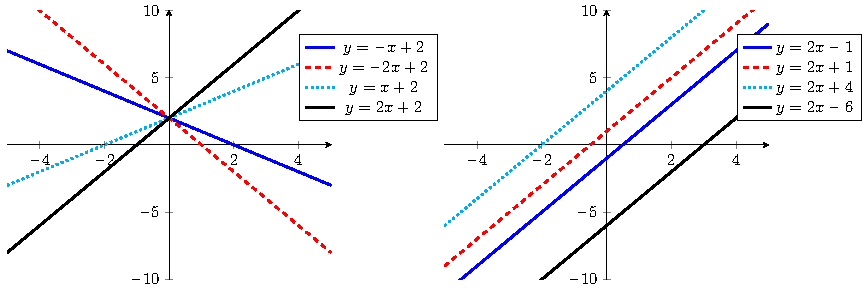
\includegraphics[width=0.9\columnwidth]{figures/0-1-fig5.pdf}
    \caption{Several members of the family of linear functions $f(x) = mx+2$ (left) and
    the family $f(x) = 2x+b$ (right).}
    \label{fig:0.1.fam1}
\end{figure}

\begin{activity}\label{A:0.1.4}
Write the equation of the line with the given information.
\ba
\item Write the equation of a line parallel to the line $y=\frac{1}{2}x+3$ passing through
    the point $(3,4)$.
\item Write the equation of a line perpendicular to the line $y=\frac{1}{2}x + 3$ passing
    through the point $(3,4)$.
\item Write the equation of a line with $y$-intercept $(0,-3)$ that is perpendicular to
    the line $y=-3x-1$.
\ea
\end{activity}\aftera




\begin{summary}
\item A function assigns one $y$ value to each $x$ value.
\item The slope of a linear function can be written as 
    \[ m = \frac{\text{Rise}}{\text{Run}} = \frac{y_2 - y_1}{x_2 - x_2} \]
\item A linear function can be written in the forms
    \[ y = mx + b \quad \text{or} \quad y-y_1 = m(x-x_1) \]
\item When examining linear data, the differences between successive $y$-values reveals
    the slope.
\end{summary}

\nin \hrulefill

\begin{exercises} 

\item (modified from NCTM Illuminations) The table below displays data that relate the number of oil changes per year and the
    cost of engine repairs.  To predict the cost of repairs from the number of oil
    changes, use the number of oil changes as the $x$ variable and the engine repair cost
    as the $y$ variable.  
    \begin{center}
        \begin{tabular}[h!]{|c|c|}
            \hline
            Oil Changes Per Year & Cost of Repairs (\$) \\ \hline \hline
            3 & 300 \\ 
            5 & 300 \\ 
            2 & 500 \\
            3 & 400 \\ 
            1 & 700 \\
            4 & 400 \\
            6 & 100 \\
            4 & 250 \\ 
            3 & 450 \\
            2 & 650 \\
            0 & 600 \\ 
            10 & 0 \\
            7 & 150 \\ \hline
        \end{tabular}
    \end{center}

    \ba
    \item Using graph paper make a plot of the data on appropriate axes.
    \item Do the data appear linear?  Why or why not?
    \item Pick two representative points from the data and use them to write the
        equation of a line that {\it fits} the data.  Plot your line on top of your data
        and discuss how well your line fits the
        data.   (This may take a few attempts.)
    \item Despite how well your data fit a linear model, it is not entirely sensible to
        use a linear model for this data.  Why?
    \ea
    
\begin{exerciseSolution}
\end{exerciseSolution}


\item The population of a city, $P$, in millions, is a function of $t$, the number of
    years since 1960, so $P = f(t)$.  Which of the following statements explains the
    meaning of $f(38) = 8$ in terms of the population of this city?
    \ba
        \item The population of this city in the year 38 is 8 million people.
        \item The population of this city in the year 8 is 38 million people.
        \item The population of this city in the year 1968 is 38 million people.
        \item The population of this city in the year 1998 is 8 million people.
    \ea
\begin{exerciseSolution}
    The independent variable is the number of years after 1960 so the ``38'' represents
    the year 1998.  Hence, the phrase ``The population of this city in the year 1998 is 8
    million people'' is the correct phrase.
\end{exerciseSolution}

\item Determine the slope and $y$-intercept of the line whose equation is $-4y + 6x + 8 =
    0$.

\begin{exerciseSolution}
    Solving for $y$ we see that 
    \[ 4y = 6x + 8 \quad \implies \quad y = \frac{6}{4} x + 2. \]
    Therefore the slope is $m=\frac{6}{4} = \frac{3}{2}$ and the $y$-intercept is $2$.
\end{exerciseSolution}

\item The value of a car in 1990 is \$13,100 and the value is expected to go down by \$80
    per year for the next 7 years.  Write a linear function for the value, $V$, of the
    1990 car as a function of the number of years from 1990, $x$.  

\begin{exerciseSolution}
    \[ V(x) = -80x + 13100 \] 
\end{exerciseSolution}
\end{exercises}
\afterexercises







\clearpage

